\section{Theoretical Background}\label{body_theoretical_background}
This chapter serves as a reference for the theoretical background necessary to understand the insights gained in the following experimental chapters.
Section \ref{theoretical_classification} discusses classification models used to train on the extended dataset resulting from the generative augmentation process. In it, \textit{Neural Networks} (NNs) for image classification are introduced and the baselines for later comparisons are examined.
Sections \ref{theoretical_da} and \ref{theoretical_gda} establish the foundation for data augmentation and generative data augmentation.
Following sections \ref{theoretical_gan}, \ref{theoretical_dcgan}, \ref{theoretical_cgan}, and \ref{theoretical_madgan} provide theoretical knowledge necessary to understand the GAN architectures and their differences. The narrative follows their increasing complexity, starting from vanilla GANs, moving through deep convolutional GANs and conditional GANs, before diving into the background of multi-agent diverse GANs.
The final section (\ref{theoretical_image_scores}) explains the theory behind the Inception Score and Fréchet Inception Distance, concluding with an examination of the state-of-the-art \textit{InceptionV3} model used to compute them.
% ########################################################################################################
% # START: IMAGE CLASSIFICATION MODELS
% ########################################################################################################
\subsection{Image Classification Models}\label{theoretical_classification}
\subsubsection{Neural Networks for Classification}
Convolutional Neural Networks (CNNs) have become the dominant architecture for image classification tasks due to their inherent ability to automatically learn hierarchical features from raw pixel data. At their core, CNNs are build up by a sequence of convolutional-, pooling- and fully connected layers to extract hierarchical features, and funneling the information, typically into the \(N\) classes defined by the training data. Convolutional layers employ learnable filters to detect local patterns in the two-dimensional information - two dimensional in the case of images specifically. Pooling layers reduce the spatial dimensions to small translations. Fully connected layers then map the extracted information into class probabilities, utilizing the \textit{Softmax} activation function. The afore mentioned layers are discussed in greater detail, in the following subsections.

\vspace{1em}

\textbf{Convolutional Layers}\label{theoretical_classification_conv_layers}
These layers compute the output from the local regions of the input. Let $(r \times c)$ be the two-dimensional input, e.g., a grayscale image, where $r$ represents the X-coordinate and $c$ the Y-coordinate of a pixel. Thus, $r \cdot c$ denotes the size of the image. Furthermore, let $(a \times b)$ be a filter with kernel size $a \cdot b$, where the filter is smaller than the input. This filter is moved from the top-left to the bottom-right over the input.

In each iteration, the dot product between the respective coefficients of the input region and the coefficients of the filter is computed. This dot product is then processed by the activation function $g$, which determines how much of the feature is present. If the activation function is ReLU, for example, only positive values are retained, meaning negative responses are set to zero. The result is written to the subsequent layer.

The stride determines how far the filter is moved after each operation. For a stride of $s = 1$, the filter can be placed in $(r - a + 1)$ positions along the height and $(c - b + 1)$ positions along the width, leading to an output size of $(r - a + 1) \times (c - b + 1)$. In general, the output size in the two-dimensional case is given by:
\[
\left( \frac{r - a + s}{s} \right) \times \left( \frac{c - b + s}{s} \right).
\]
%TODO: point to the right figure
An image of this process can be found in Figure X in the Appendix (7). This image shows an input of size $[10 \times 10]$ and a filter of size $[3 \times 3]$. With a stride of $s = 1$, the resulting layer has a size of $[8 \times 8]$ (computed as $\left(10 - 3 + 1\right) \times \left(10 - 3 + 1\right)$).

The stride of the filter can also be greater than $1$. Additionally, there is the option to apply padding to the image. There are different ways to implement padding. When padding of size $p$ is applied, the output size for a square input and filter is calculated as follows:
\[
\textbf{Output size} = \left\lfloor \frac{r - a + 2p}{s} \right\rfloor + 1
\]
where $\lfloor \cdot \rfloor$ denotes the floor function, which ensures that the output size is an integer.

\vspace{1em}

\textbf{Pooling Layers}\label{theoretical_classification_pooling_layers}
A pooling layer compresses the data along the spatial axes to reduce its dimensionality. Similar to the convolutional layer, a pooling layer uses a filter that moves by the stride value. However, instead of summing the covered elements, the pooling operation applies the Max operator, selecting the maximum value within the filter's region.

For example, starting with an input of size $[32 \times 32 \times 10]$, applying a pooling operation with a $[2 \times 2]$ filter and a stride of 2 results in an output size of $[16 \times 16 \times 10]$. This operation reduces the spatial dimensions by half while keeping the depth unchanged.

Max pooling helps retain the most important features, providing some invariance to small translations or distortions in the input, which is crucial for tasks like object recognition in convolutional neural networks (CNNs).


\vspace{1em}

\textbf{Fully-Connected Layers}\label{theoretical_classification_fully_connected_layers}
Fully-Connected (FC), also called \textit{Dense} layer, typically computes the scores for the respective classes. In the case of ten classes, the result is a volume of size $[1 \times 1 \times 10]$\footnote{Typically, the output from the layer before the FC one is "flattened" into a one-dimensional vector, preserving all information but removing spatial structure. For example, a $[2 \times 2]$ layer would become a vector of size $[1 \times 4]$.}. By this stage, all spatial information has been transformed, leaving a quasi-one-dimensional vector containing the ten class scores for the CIFAR-10 dataset.

In a FC layer, each input is connected to each output, meaning every neuron in the previous layer is connected to each neuron in the FC layer. The output is the weighted sum of all inputs, followed by an activation function, leading to the final classification scores that represent the likelihood of the input belonging to each class. The spatial dimensions are collapsed into a single vector of class scores, which are then used for classification.

\textbf{Batch Normalization Layers}\label{theoretical_classification_batchnorm_layers}
With their introduction in "\textit{Batch Normalization: Accelerating Deep Network Training by Reducing Internal Covariate Shift}" by Ioffe et al. \cite{ioffe2015batchnormalizationacceleratingdeep}, Batch Normalization (batchnorm) is an integreal part of convolutional networks. These layers normalize the inputs to subsequent layers and theirby stability the distribution of activations throughout the training process. This reduces the internal covariate shift, allowing for higher learning rates and faster convergence. By normalization of activation, batchnorm helps prevent gradients from vanishing or exploding. Additionally, it can provide regularization benefits and eliminate the need for Dropout, in some cases. With the afore mentioned benefits, batchnorm layers are particularily beneficial for deep learning networks with many layers.


\textbf{Typical Activation Functions for CNNs}

\begin{itemize}
    \item \textbf{ReLU (Rectified Linear Unit)}: \label{theoretical_activations_relu}
    \begin{equation}
    g(x) = \max(0, x)
    \end{equation}
    ReLU is the most widely used activation function in CNNs. It introduces non-linearity while maintaining efficiency by outputting zero for negative values and passing positive values unchanged.

    \item \textbf{Leaky ReLU}: \label{theoretical_activations_leakyrelu}
    \begin{equation}
        f(x) =
        \begin{cases}
        0 \quad \text{if } x < 0 \\
        x \quad \text{otherwise}
        \end{cases}
    \end{equation}
    A variant of ReLU, Leaky ReLU allows small negative values to flow through, addressing the "dying ReLU" problem where neurons can become inactive.

    \item \textbf{Sigmoid (Logistic)}:  \label{theoretical_activations_sigmoid}
    \begin{equation}
        g(x) = \frac{1}{1 + e^{-x}}
    \end{equation}
    The sigmoid function squashes values between 0 and 1, commonly used for binary classification tasks. However, it can suffer from vanishing gradients for very large or small inputs.

    \item \textbf{Tanh (Hyperbolic Tangent)}:  \label{theoretical_activations_tanh}
    \begin{equation}
    g(x) = \frac{2}{1 + e^{-2x}} - 1
    \end{equation}
    Tanh outputs values between -1 and 1 and is similar to the sigmoid but with a wider output range, making it more effective in many scenarios compared to sigmoid.

    \item \textbf{Softmax}: \label{theoretical_activations_softmax}
    \begin{equation}
    g(x_i) = \frac{e^{x_i}}{\sum_{j} e^{x_j}}
    \end{equation}
    Softmax is typically used in the output layer of CNNs for multi-class classification. It converts logits into probabilities, ensuring that the sum of the outputs is 1.
\end{itemize}

\subsubsection{Classification Models for augmented Training}
The classification models, on which the data augmentation is tested, are simple CNN classifiers consisting of the described layers. For each dataset MNIST, Fashion MNIST and CIFAR10 \ref{used_datasets}, a dedicated classifier architecture is created. The main differences between these architectures is the number of blocks, made of two-dimensional \hyperref[theoretical_classification_conv_layers]{convolutional}, \hyperref[theoretical_classification_batchnorm_layers]{batchnorm} and \hyperref[theoretical_classification_pooling_layers]{pooling} layers. All three models use a use the \hyperref[theoretical_activations_relu]{ReLU} function for activation of the convolutional layers and the \hyperref[theoretical_activations_softmax]{Softmax} function for the activation at their respective output layer, resulting in probability distribution over the space of classes. More on the specifical model architectures can be found in chapter \ref{body_prelim}. %TODO: link the correct subsection
% ########################################################################################################
% # END: IMAGE CLASSIFICATION MODELS
% ########################################################################################################

% ########################################################################################################
% # START: DATA AUGMENTATION
% ########################################################################################################

\subsection[Data Augmentation - DA]{Data Augmentation}\label{theoretical_da}
In this chapter, DA techiques in the context on images are discussed is greater detail. Starting with traditional augmentations e.g. rotating or cropping an image, ending on generative augmentations for which generative models are used to expand the training data of subsequent models.

\subsubsection[Traditional Data Augmentation - TDA]{Traditional Data Augmentation}\label{theoretical_tda}
The need for data augmentation to make classification algorithms more resillient exists ever since. Early papers, mentioning the augmentation of data for classification tasks date back to the 70's \cite{Nagy1966}.For the context of deep learning however, the augmentation of images was popularized by Krizhevsky et al. in 2012 \cite{Krizhevsky2012traditionaldataaugmentation}, with the introduction of the \textit{AlexNet} - a deep CNN, to classify the images from the \textit{ImageNet} \cite{ImageNetDataset5206848} dataset, with 1000 classes. Although this paper too mentioned the work of Simard et al. from 2003 \cite{Simard2003bestpracticesforcnns}.

Generally speaking, traditional data augmentation techiques can be described as enlarging initial training data by transformations preserving respective labels of single instances. These techiques soley focus on already existing data, without creating entirely new instances (see: \ref{theoretical_gda}). Such augmentations are categorized, based on their type of altering transformations:

\noindent\textit{Geometric Augmentation}\\
This category of augmentations modify the shape, position and perspective: Rotation, Scaling, Flipping, Cropping, Shearing, Perspective Transform.

\noindent\textit{Photometric Augmentation}\\
Altering the pixel values while keeping the spatial structure: Brightness, Contrast, Hue Shift, Blurring.

\noindent\textit{Noise-Corruption Augmentation}\\
Imitating real-world degradations and distorions of cameras and sensors: Gaussion Noise, Speckle Noise, Salt-and-Pepper Noise.\\

\begin{figure}[htbp]
    \centering
    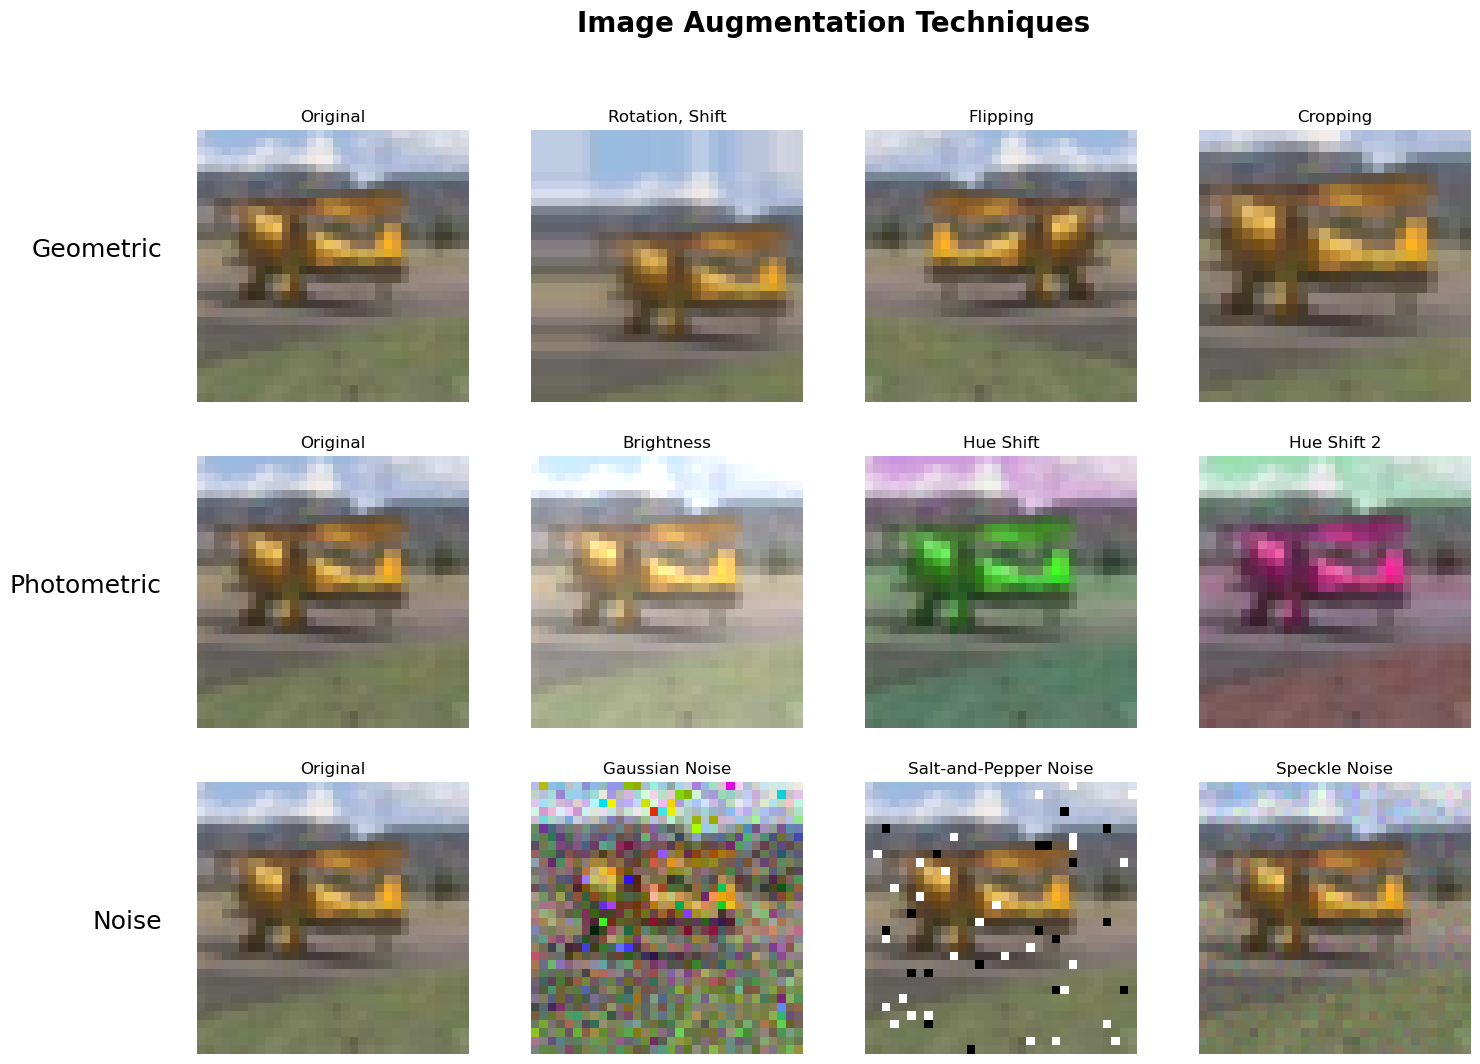
\includegraphics[width=.9\textwidth]{abb/traditional_image_augmentation_examples.png}
    \caption{Examplary use of traditional augmentation techniques from the categories \textit{geomentric} (first row), \textit{photometric} (second row) and \textit{noice-corruption} third row.}
    \label{fig:figure_tda_examples}
\end{figure}

\noindent
When applying the augmentations shown in Figure~\ref{fig:figure_tda_examples}, its mandatory to keep domain specific knowledge and constraints in mind. Flipping images originating from the MNIST dataset to train a generative model can result in an image, showing a horizontally flipped 9 which, in the domain of arabic numbers, is semantically false. Having to classify a plain, that can have differing shapes, colors three-dimensional orientations in space and images takes by a dusted lense, applying all of the above augmentations could be beneficial.

\subsubsection[Generative Data Augmentation - GDA]{Generative Data Augmentation}\label{theoretical_gda}
Differing from the previously mentioned TDA \ref{theoretical_tda}, GDA does not focus on altering existing data instances but rather on creating entirely new samples that match the underlying data distribution of the training data. These generated instances may or may not include labels.

The goal is to train a generative model \( G \) that produces instances \( X_1 \), for example, from a noise vector \( z \), such that the distribution of the generated data approximates the true distribution \( P(X) \) of the original dataset. In this context, \( G \) can be viewed as a function:

\[
G: z \mapsto X_1, \quad X_1 \sim P_G(X) \approx P(X),
\]

\noindent
where \( P_G(X) \) is the learned distribution of the generative model, aiming to approximate the real data distribution \( P(X) \).

In the case of \textit{conditional} generative data augmentation, additional information such as class labels \( y \) is incorporated into the generation process. This allows the model to generate samples corresponding to specific categories within the data. The conditional generative model \( G \) then follows:

\[
G: (z, y) \mapsto X_1, \quad X_1 \sim P_G(X \mid y) \approx P(X \mid y),
\]

\noindent
where \( P_G(X \mid y) \) represents the learned conditional distribution, aiming to approximate the real class-conditioned data distribution \( P(X \mid y) \). This enables targeted data generation for specific categories, enhancing data diversity while maintaining class consistency.

% ########################################################################################################
% # END: DATA AUGMENTATION
% ########################################################################################################



% ########################################################################################################
% # START: Generative Aderserial Networks
% ########################################################################################################

\subsection[Generative Adversarial Network - GAN]{Generative Adversarial Network}\label{theoretical_gan}
\subsubsection{Challenges in GAN Training}
\paragraph[Mode Collapse]{Mode Collapse}
\paragraph[Training Instability]{Training Instability}
\paragraph[Evaluation Difficulties]{Evaluation Difficulties}

\subsection[Deep Convolutional Generative Adversarial Network - DCGAN]{Deep Convolutional Generative Adversarial Network}\label{theoretical_dcgan}

\subsection[Conditional Generative Adversarial Network - cGAN]{Conditional Generative Adversarial Network}\label{theoretical_cgan}

\subsection[Multi-Agent Diverse Generative Adversarial Network - MADGAN]{Multi-Agent Diverse Generative Adversarial Network}\label{theoretical_madgan}

% ########################################################################################################
% # END: Generative Aderserial Networks
% ########################################################################################################


% ########################################################################################################
% # START: Image Scores
% ########################################################################################################

\subsection{Image Scores}\label{theoretical_image_scores}
\subsubsection[Inception Score - IS]{Inception Score}
\subsubsection[Fréchet Inception Distance - FID]{Fréchet Inception Distance}
\subsubsection[InceptionV3 Model]{InceptionV3 for Image Evaluation}

% ########################################################################################################
% # START: Image Scores
% ########################################################################################################









\newpage
